% !TEX root = ../ac_paper.tex

\section{Isolated components and neighborhood sizes}\label{sec:isolated}

\subsection{Isolated components}

In \autoref{ss:greedy_search}, we explored a greedy approach to finding AC-trivializations of a presentation \(\pi\).
Specifically, the goal was to construct a sequence of presentations \((\pi_0, \dots, \pi)\), where \(\pi_0\) is the trivial presentation, such that each consecutive pair in the sequence is related by an AC move.
Furthermore, at each step \(k\), the presentation \(\pi_k\) was chosen to have the shortest possible length among all presentations connected to \(\pi_{k+1}\) via an AC move.
In general, the length of a presentation in an AC-trivialization tends to exceed the length of the original presentation being trivialized.
The minimum increase in length across all possible AC-trivializations serves as an invariant of the presentation.
We will explore this invariant using concepts from persistent homology.

\subsubsection{Formalization}

A \textit{based graph} is a pair $(\Gamma, v_0)$ consisting of a graph $\Gamma$ and a preferred vertex $v_0$ in it.
We will often drop $v_0$ from the notation.
A \textit{based subgraph} $\Gamma_n$ of $\Gamma$, written $\Gamma_n \leq \Gamma$, is a subgraph $\Gamma_n$ of $\Gamma$ with the same preferred vertex.
We say that $\Gamma_n$ is \textit{full} in $\Gamma$ if for any two vertices in $\Gamma_n$ joined by an edge in $\Gamma$, the edge is also in $\Gamma_n$.
A \textit{filtration} of a based graph $\Gamma$ is a collection
\[
\Gamma_0 \leq \Gamma_1 \leq \Gamma_2 \leq \dotsb
\]
of based subgraphs of $\Gamma$ for which each vertex and edge of $\Gamma$ is in $\Gamma_n$ for some $n$.
We refer to $\Gamma$ as a \textit{filtered based graph}.
If each $\Gamma_n$ is full in $\Gamma$ we refer to the filtration as full and notice that full filtrations are equivalent to $\N$ valued functions from the set of vertices of $\Gamma$ sending $v_0$ to $0$.

Let $\Gamma^{\text{AC(k)}}$ be the graph whose vertices are $k$-balanced presentations, based at the trivial presentation, having an edge between two vertices if there is an AC move between them.
Additionally, $\Gamma^{\text{AC(k)}}$ is equipped with a full filtration obtained from the function sending a vertex to the length of its presentation minus $k$.

%\subsubsection{Isolation values and isolated components}

Given a filtered based graph $(\Gamma, v_0)$.
The \textit{filtration value} $\Filt(v)$ of a vertex $v$ is the smallest $n \in \N$ such that $v$ is a vertex in $\Gamma_n$.
Similarly, its \textit{connectivity value} $\Conn(v)$ is the smallest $n \in \N$ such that $v$ and $v_0$ can be joined by a path in $\Gamma_n$ or is set to $\infty$ if such path does not exist in $\Gamma$.

The \textit{isolation value} of a vertex $v$ in a filtered based graph is defined as
\[
\Isol(v) = \Conn(v) - \Filt(v),
\]
a number in $\N \cup \set{\infty}$.
A vertex is said to be \textit{isolated} if its isolation value is positive.

We introduce an equivalence relation on isolated vertices.
Two belong to the same \textit{isolated component} if they have the same connectivity value, say $n$, and they can be joined by a path in $\Gamma_{n-1}$.
The \textit{isolation value} of a component is the maximum of the isolation values of its elements.

We can interpret these invariants using the framework of topological data analysis, see for example \cite{carlsson2022tda}.
Specifically, the set of isolated components of a based filtered graph $\Gamma$ corresponds to the multiset of bars in the barcode of its reduced persistent $0$-homology.
Additionally, the isolation value of an isolated component corresponds to the length of its associated bar.

\subsubsection{Experimental results}

Let \(\Gamma^\ell\) be the full subgraph of \(\Gamma^{\text{AC(2)}}\), with the induced filtration, consisting of all presentations with a connectivity value less than or equal to \(\ell\).
Explicitly, \(\Gamma^\ell\) includes all vertices that can be connected to the trivial vertex via paths containing only presentations of length at most \(\ell\).

We will denote by $v(\ell)$ and $e(\ell)$ the number of vertices and edges of $\Gamma^\ell$.
Let us denote by $ic(\ell)_k$ the number of isolated components with isolation value $k$.
\autoref{fig:classical_persistence} summarize our results for the classic AC moves whereas \autoref{fig:prime_persistence} does so for their prime version.\footnote{For this task we used \texttt{giotto-TDA} version 5.1 \cite{tauzin2021giotto}.
	Specifically, its binding of the \texttt{SimplexTree} data structure introduced in \cite{boissonnat2014simplex} and implemented in \texttt{GUDHI} \cite{maria2014gudhi}.}

\begin{figure}
	\begin{tabular}{|c|c|c|c|c|c|}
		\hline
		$\ell$ & $v(\ell)$ & $e(\ell)$ & $ic(\ell,1)$ & $ic(\ell,2)$ & $ic(\ell,3)$ \\ \hline
		3 & 36 & 72 & 0 & 0 & 0 \\ \hline
		4 & 100 & 248 & 0 & 0 & 0 \\ \hline
		5 & 388 & 1072 & 0 & 0 & 0 \\ \hline
		6 & 884 & 2376 & 0 & 0 & 0 \\ \hline
		7 & 3892 & 10775 & 0 & 0 & 0 \\ \hline
		8 & 9172 & 25675 & 0 & 0 & 0 \\ \hline
		9 & 37428 & 106513 & 0 & 0 & 0 \\ \hline
		10 & 84996 & 239733 & 0 & 0 & 0 \\ \hline
		11 & 350356 & 1002439 & 4 & 0 & 0 \\ \hline
		12 & 791140 & 2251375 & 16 & 0 & 0 \\ \hline
		13 & 3238052 & 9321629 & 72 & 4 & 0 \\ \hline
		14 & 7199908 & 20573343 & 144 & 4 & 0 \\ \hline
        15 & ? & ? & ? & ? & ? \\ \hline
        16 & 64623652 & 185162236 & 1034 & 88 & 20 \\ \hline
	\end{tabular}
	\caption{Classical AC moves}
	\label{fig:classical_persistence}
\end{figure}

\begin{figure}
	\begin{tabular}{|c|c|c|c|c|c|}
		\hline
		$\ell$ & $v(\ell)$ & $e(\ell)$ & $ic(\ell,1)$ & $ic(\ell,2)$ & $ic(\ell,3)$ \\ \hline
		3 & 36 & 40 & 3 & 0 & 0 \\ \hline
		4 & 100 & 152 & 3 & 0 & 0 \\ \hline
		5 & 388 & 712 & 3 & 0 & 0 \\ \hline
		6 & 884 & 1528 & 3 & 0 & 0 \\ \hline
		7 & 3892 & 6984 & 3 & 0 & 0 \\ \hline
		8 & 9172 & 16728 & 3 & 0 & 0 \\ \hline
		9 & 37428 & 69752 & 3 & 0 & 0 \\ \hline
		10 & 84996 & 155752 & 3 & 0 & 0 \\ \hline
		11 & 350356 & 655928 & 19 & 0 & 0 \\ \hline
		12 & 791140 & 1467080 & 67 & 0 & 0 \\ \hline
		13 & 3238052 & 6107112 & 243 & 16 & 0 \\ \hline
		14 & 7199908 & 13414744 & 483 & 16 & 0 \\ \hline
        15 & 29243812 & 55306744 & 1819 & 136 & 32 \\ \hline
        16 & 64623652 & 120824232 & 3923 & 208 & 80 \\ \hline
    \end{tabular}
	\caption{Prime AC moves}
	\label{fig:prime_persistence}
\end{figure}

%\[
%%OLD
%\begin{tabular}{|c|c|c|c|c|c|}
%	\hline
%	$\ell$ & $v(\ell)$ & $e(\ell)$ & $ic(\ell,1)$ & $ic(\ell,2)$ & $ic(\ell,3)$ \\ \hline
%	2 & 4 & 4 & 0 & 0 & 0 \\ \hline
%	3 & 36 & 76 & 0 & 0 & 0 \\ \hline
%	4 & 100 & 241 & 0 & 0 & 0 \\ \hline
%	5 & 388 & 1027 & 0 & 0 & 0 \\ \hline
%	6 & 876 & 2224 & 0 & 0 & 0 \\ \hline
%	7 & 3844 & 10057 & 0 & 0 & 0 \\ \hline
%	8 & 8992 & 23726 & 0 & 0 & 0 \\ \hline
%	9 & 35844 & 97243 & 0 & 0 & 0 \\ \hline
%	10 & 81004 & 216412 & 1 & 0 & 0 \\ \hline
%	11 & 338020 & 920347 & 6 & 3 & 0 \\ \hline
%	12 & 762116 & 2043028 & 12 & 8 & 1 \\ \hline
%	13 & 3115928 & 8478633 & 32 & 21 & 2 \\ \hline
%\end{tabular}
%\]

\subsection{Neighborhoods}

Let us return to our data set of 1190 presentations in the Miller–Schupp series for \(n \leq 7\) and \(\length(w) \leq 7\).
Using the methods described in \autoref{sec:ppo}, we trained a PPO agent that successfully solved 417 of these presentations. We will refer to the set of these 417 presentations as PPO-solved and the remaining 773 presentations as PPO-unsolved.
Our goal is to analyze the relationship between these labels and the sizes of their respective AC neighborhoods.
A presentation is considered to be in the \(k\)-step neighborhood of another if they can be connected by applying at most \(k\) AC moves.

\subsubsection{Experimental results}

There are 131 distinct neighborhood sizes in our data.
Their basic statistics are
\[
\begin{tabular}{cccccc}
	\toprule
	\textbf{Min} & \textbf{Max} & \textbf{Mean} & \textbf{Median} \\
	\midrule
	72,964 & 89,872 & 89,532 & 89,859 \\
	\bottomrule
\end{tabular}
\]
A more detailed description of the frequency of values is presented in \autoref{fig:prime_combined_pie}.

\begin{figure}
	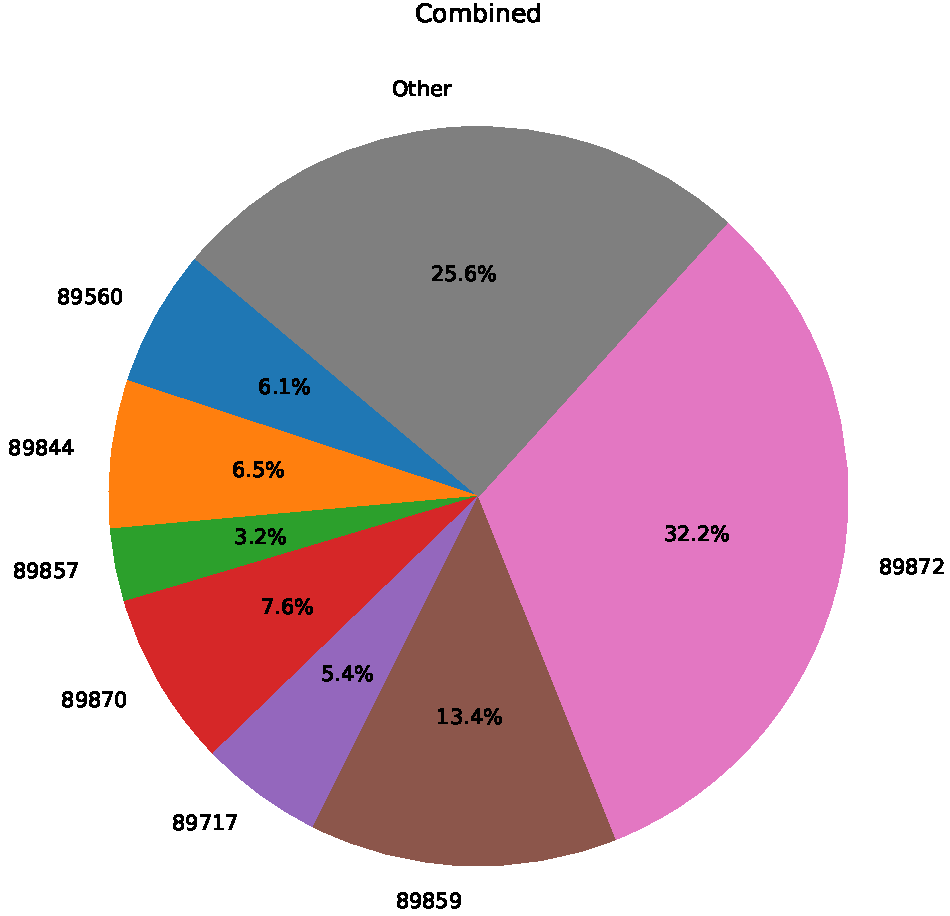
\includegraphics[scale=.4]{fig/prime_combined_pie_rl_cropped.pdf}
	\caption{Sizes of the 5-step neighborhood of all considered presentations in the Miller–Schupp series. We group neighborhood sizes whose representation is below 2.5\%.}
	\label{fig:prime_combined_pie}
\end{figure}

The largest neighborhood size accounts for nearly a third of all considered presentations.
However, it represents only 2.4\% of PPO-solved presentations, while constituting almost half (48.3\%) of the PPO-unsolved presentations.
For more details, please refer to \autoref{fig:prime_pies}.

In contrast, using BFS, these proportions are 7.1\% and 52.5\%, respectively.

Another notable feature visible in \autoref{fig:prime_pies} is that just three neighborhood sizes account for over three-quarters of all PPO-unsolved presentations.
When considering six neighborhood sizes, this proportion rises to 96.9\%.
In fact, only twelve neighborhood sizes are present among PPO-unsolved presentations, whereas all 131 sizes appear among PPO-solved presentations.
The most common neighborhood size for PPO-solved presentations is 89,560, representing only 17.3\% of them.
Moreover, 54.2\% of all PPO-solved presentations have a neighborhood size shared by less than 2.5\% of other PPO-solved presentations.

\begin{figure}
	\centering
	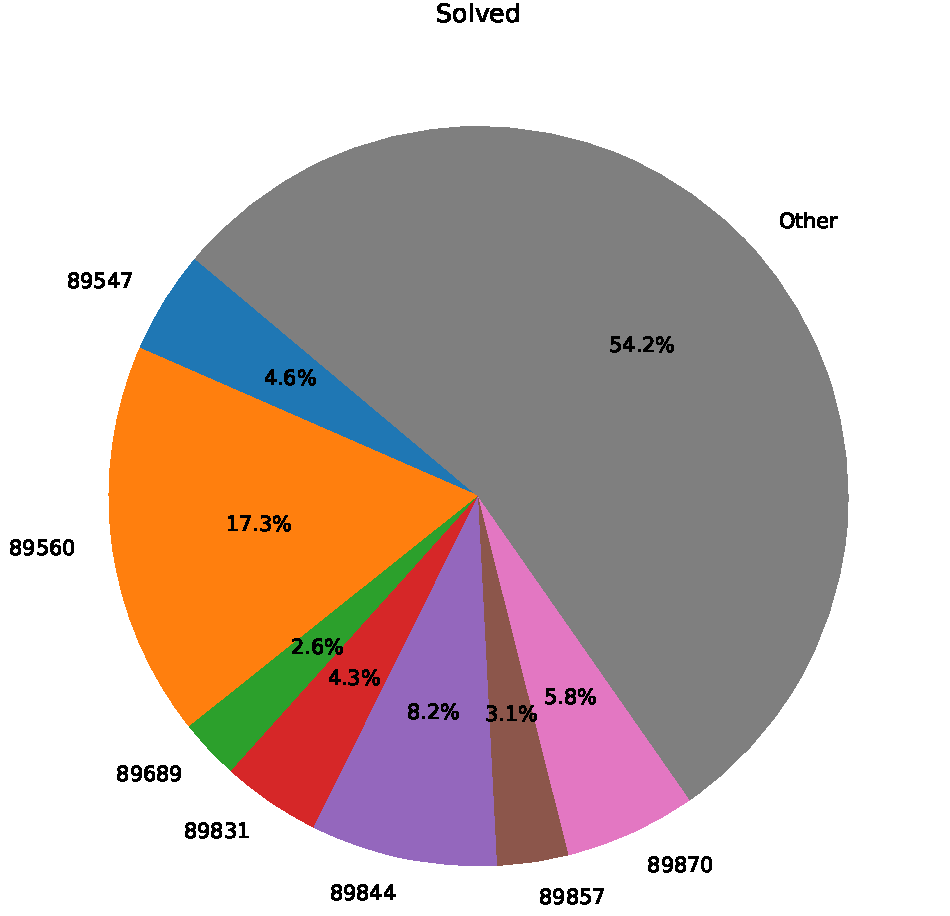
\includegraphics[scale=.35]{fig/prime_solved_pie_rl_cropped.pdf}
	\ 
	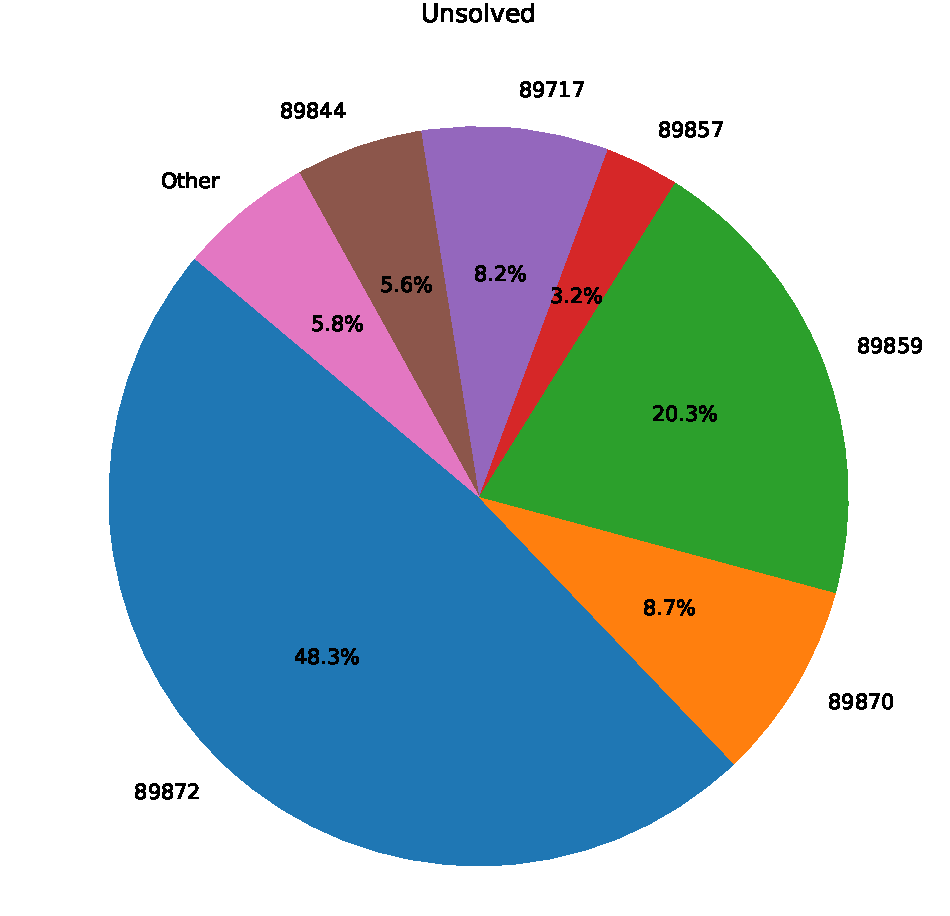
\includegraphics[scale=.35]{fig/prime_unsolved_pie_rl_cropped.pdf}
	\caption{Pie charts for the neighborhood size of PPO-solved and PPO-unsolved presentations. We grouped sizes with representation below 2.5\%.}
	\label{fig:prime_pies}
\end{figure}

As we observed, having a maximal neighborhood size provides significant insight into whether a presentation is labeled as PPO-solved or PPO-unsolved.
Additionally, the minimum neighborhood size among PPO-unsolved presentations—89,573—is also quite telling, as 54\% of PPO-solved presentations have neighborhood sizes smaller than this value.
This percentage can be further improved by considering that the neighborhood sizes of PPO-unsolved presentations are concentrated within three specific bands.
Please refer to \autoref{fig:prime_histogram} for more details.
We find that 64.3\% of PPO-solved presentations fall outside the three bands \([89,575, 89,575]\), \([89,715, 89,831]\), and \([89,844, 89,872]\), which together contain over 99\% of PPO-unsolved presentations.
By narrowing the last band to \([89,859, 89,872]\), these three bands now encompass the neighborhood sizes of over 90\% of PPO-unsolved presentations, while their complement includes 77.2\% of PPO-solved presentations.


\begin{figure}
	\centering
	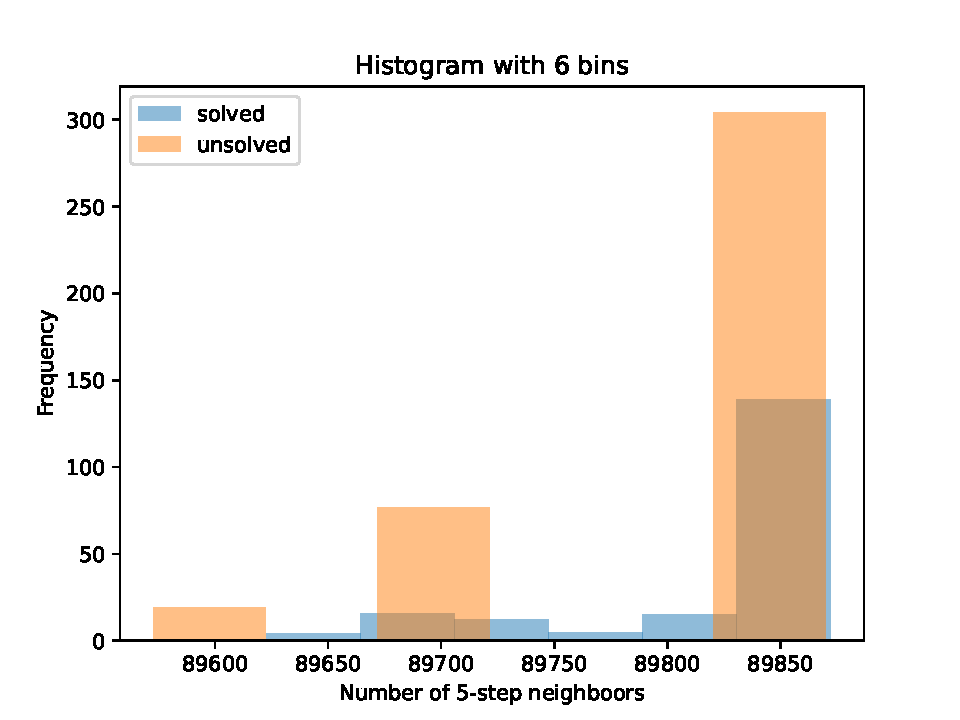
\includegraphics[scale=.34]{fig/prime_histogram_rl.pdf}
	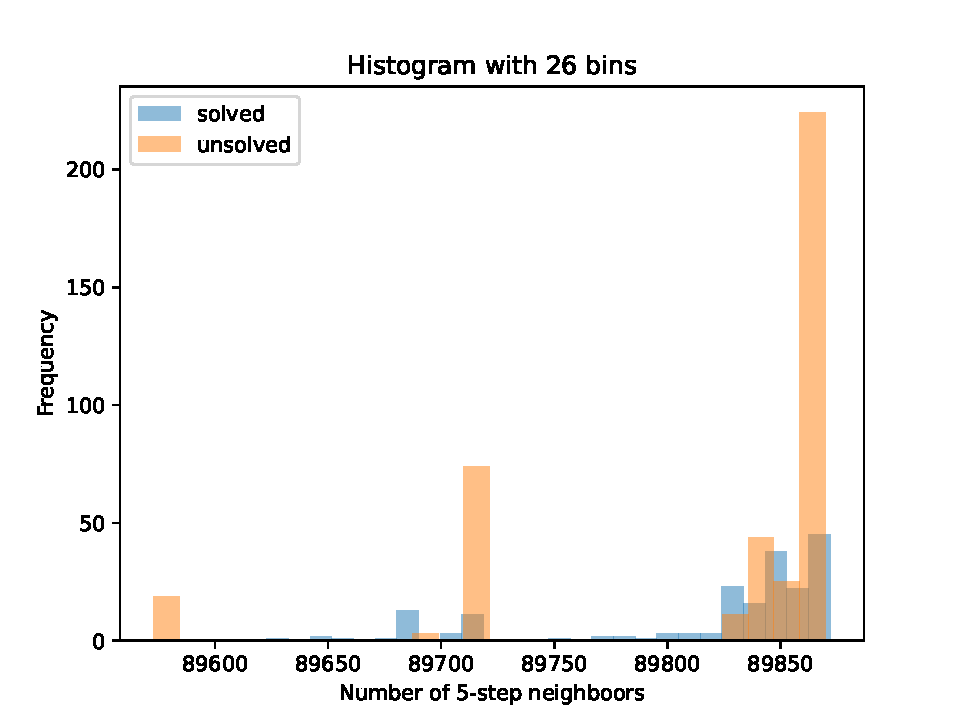
\includegraphics[scale=.34]{fig/prime_histogram_rl2.pdf}
	\caption{Histograms with 6 and 26 bins respectively of the neighborhood sizes of the 417 PPO-solved and 773 PPO-unsolved presentations.}
	\label{fig:prime_histogram}
\end{figure}

\medskip

One might expect that enhancing the discriminatory power of \(n\)-neighborhoods could be achieved by incorporating features beyond their size.
We explored two additional types of features, but surprisingly, they only marginally improved the accuracy of PPO-solved/unsolved predictions.
The first type was based on node centrality, while the second focused on spectral features of the neighborhood graphs.
The latter was particularly intriguing, given the emphasis on Markov processes and the well-known relationship between random walks on graphs and the graph Laplacian.
